%
%	Configure LaTeX to produce a PDF presentation using the beamer class
%

\documentclass[ignorenonframetext,11pt]{beamer}
\usepackage[ngerman]{babel}
\usepackage[utf8]{inputenc}		% For UTF-8 support
\usepackage[T1]{fontenc}

\usepackage{graphicx}


\usepackage{beamerthemesplit}
\usepackage{patchcmd}
\usepackage{tabulary}		% Support longer table cells
\usepackage{booktabs}		% Support better tables
\usepackage[sort&compress]{natbib}

\usepackage{framed}			% Allow background color for images
\definecolor{shadecolor}{named}{white}


\usepackage{subfigure}

\let\oldSubtitle\subtitle


% Configure default metadata
\input{mmd-default-metadata}


%\AtBeginSection[]
%{
 %\begin{frame}
    %\frametitle{Inhalt}
	%\tableofcontents %[currentsection,currentsubsection]
   %\end{frame}
%}


\long\def\citefoot#1{\let\thefootnote\relax\footnotetext{\citet{#1}} }

\def\mytitle{File Network: Strukturdesign}
\def\myauthor{Anastasia Kazakova, Bengt Lüers}
\def\latexmode{beamer}
\def\latexxslt{beamer}
\def\theme{keynote-IntSysTheme}
\input{mmd-natbib-plain}
%
%	Get ready for the actual document
%

%
% Use default MMD metadata for beamer equivalents
%

\ifx\subtitle\undefined
\else
	\oldSubtitle{\subtitle}
\fi

\ifx\affiliation\undefined
\else
	\institute{\affiliation}
\fi

\ifx\mydate\undefined
	\def\mydate{\today}
\else
	\date{\mydate}
\fi

\ifx\event\undefined
\else
	\date[\mydate]{\mydate~ / \event }
\fi


%\input{mmd-title}

% Show "current/total" slide counter in footer
\title[\mytitle\hspace{2em}\insertframenumber/
\inserttotalframenumber]{\mytitle}


\author{\myauthor}
\addtolength{\parskip}{\baselineskip}

\ifx\theme\undefined
\else
	\usetheme{\theme}
\fi

\begin{document}
\frame[plain]{\setlength\parskip{0pt}\titlepage}

\# \#

\section{Erarbeiten des Strukturdesigns}
\label{erarbeitendesstrukturdesigns}

\begin{frame}

\frametitle{Schritt eins}
\label{schritteins}

\textbf{Brainstorming}

\begin{itemize}
\item Kreisen

\item Farben

\item Venn-Diagramme

\end{itemize}

\textbf{State of the Art}

\begin{itemize}
\item Informationsvisualisierung

\item Bäume

\item Graphen

\end{itemize}

\end{frame}

\begin{frame}

\frametitle{Schritt eins: Beispiele}
\label{schritteins:beispiele}

\begin{figure}[htbp]
\centering
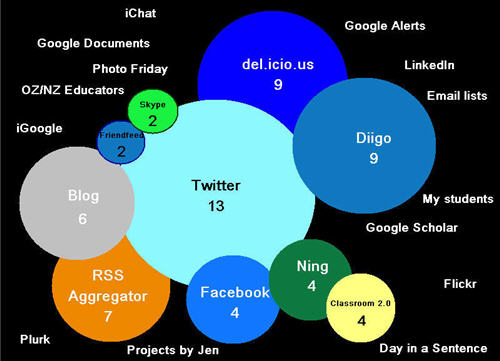
\includegraphics[keepaspectratio,width=\textwidth,height=0.75\textheight]{s1_bsp1.jpg}
\caption{Beispiel 1}
\label{}
\end{figure}


\end{frame}

\begin{frame}

\frametitle{Schritt eins: Beispiele}
\label{schritteins:beispiele}

\begin{figure}[htbp]
\centering
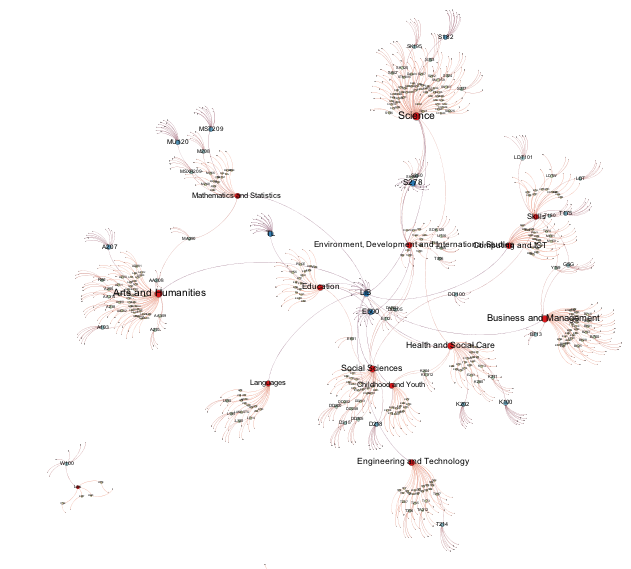
\includegraphics[keepaspectratio,width=\textwidth,height=0.75\textheight]{s1_bsp2.png}
\caption{Beispiel 2}
\label{}
\end{figure}


\end{frame}

\begin{frame}

\frametitle{Schritt eins: Beispiele}
\label{schritteins:beispiele}

\begin{figure}[htbp]
\centering
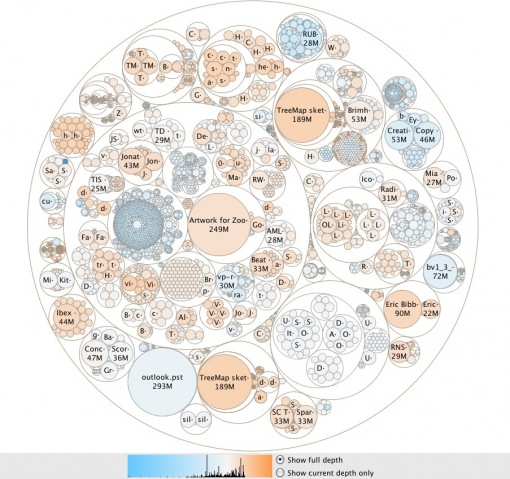
\includegraphics[keepaspectratio,width=\textwidth,height=0.75\textheight]{s1_bsp3.jpg}
\caption{Beispiel 3}
\label{}
\end{figure}


\end{frame}

\begin{frame}

\frametitle{Schritt zwei}
\label{schrittzwei}

\textbf{Frag mal die Anderen}

\begin{itemize}
\item Bunte Stifte

\item Paar Elemente

\begin{itemize}
\item Kreise

\item Tags

\item Verbindungen

\end{itemize}

\item Aufgaben

\end{itemize}

\end{frame}

\section{Kunststunde}
\label{kunststunde}

\begin{frame}

\frametitle{Ziele}
\label{ziele}

\begin{itemize}
\item Ideen sammeln

\item Schauen, ob unsere Ideen ankommen

\item Entdecken neuer Blickwinkel

\end{itemize}

\end{frame}

\begin{frame}

\frametitle{Vorgehen}
\label{vorgehen}

\begin{itemize}
\item 6 Aufgaben

\item 2 Aufbaus

\begin{itemize}
\item Dateikärtchen

\item Papier

\item Stifte

\item Papierelemente

\begin{itemize}
\item Kreise

\item Tags

\item Verbindungen

\end{itemize}

\end{itemize}

\end{itemize}

\end{frame}

\begin{frame}

\frametitle{Ideen}
\label{ideen}

\begin{figure}[htbp]
\centering
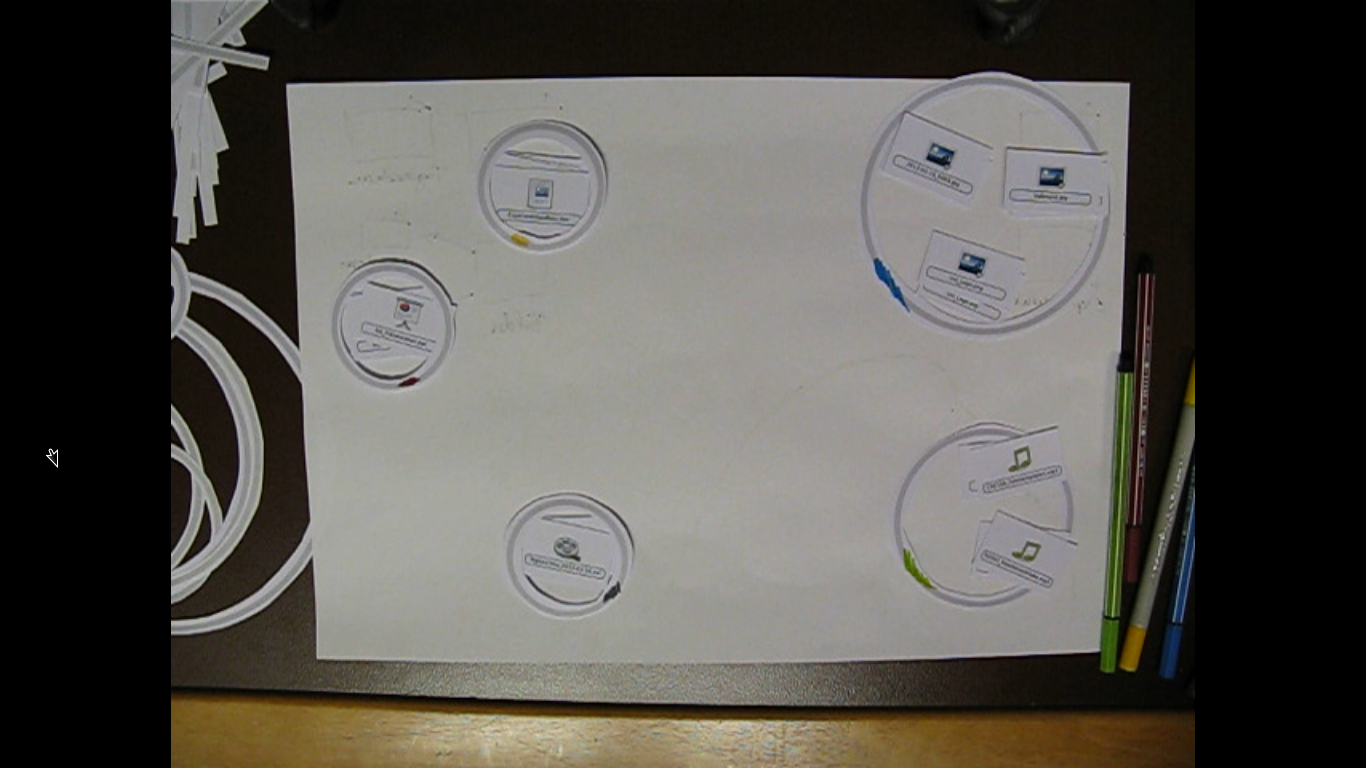
\includegraphics[keepaspectratio,width=\textwidth,height=0.75\textheight]{1_-_Kreise_fuer_mehrere_und_einzelne_Stacks.png}
\caption{Kreise für mehrere und einzelne Stacks}
\label{}
\end{figure}


\end{frame}

\begin{frame}

\frametitle{Ideen}
\label{ideen}

\begin{figure}[htbp]
\centering
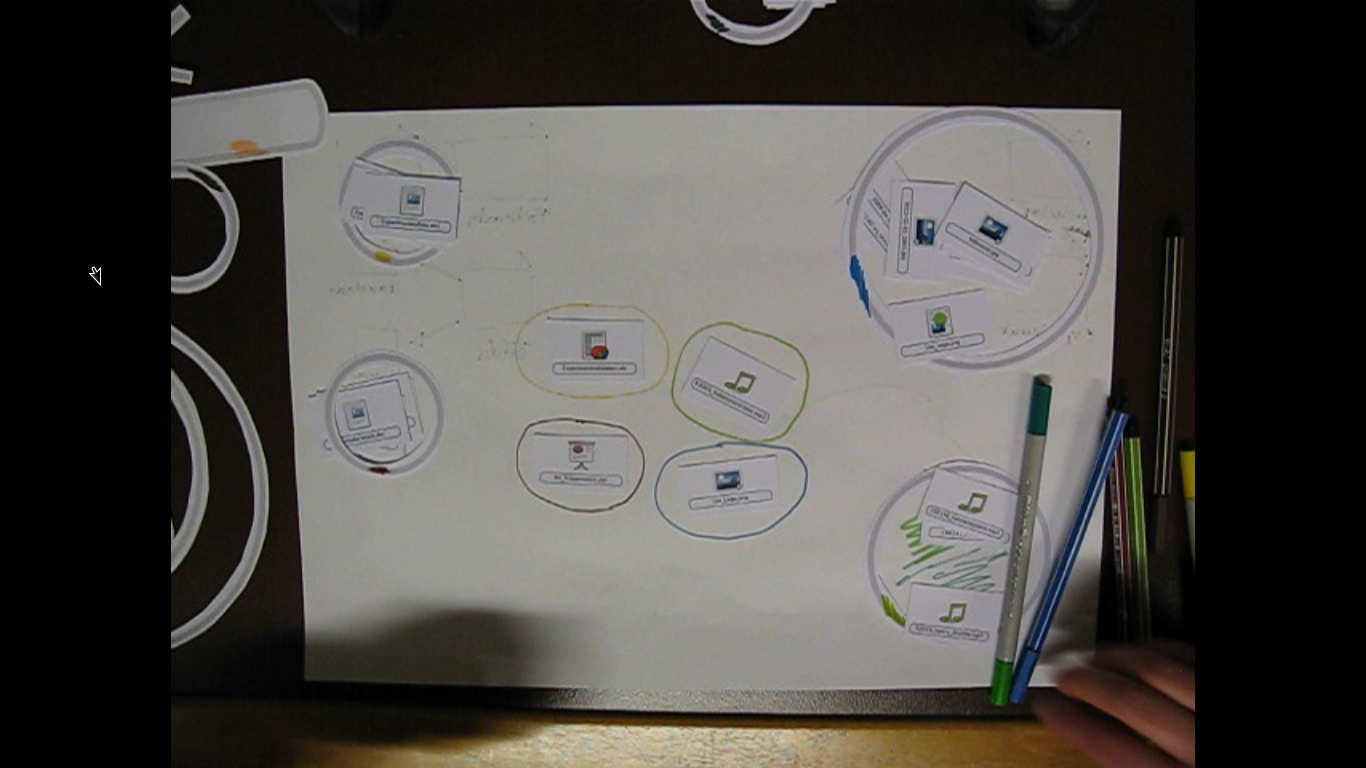
\includegraphics[keepaspectratio,width=\textwidth,height=0.75\textheight]{Angy_-_Farbige_Umrandungen_einzelner_Dateien.png}
\caption{Farbige Umrandungen einzelner Dateien}
\label{}
\end{figure}


\end{frame}

\begin{frame}

\frametitle{Ergebnisse}
\label{ergebnisse}

\textbf{Überschneidungen}

\begin{itemize}
\item Kreise sind toll

\item Farben spiele eine Rolle

\end{itemize}

\textbf{Neue Ideen}

\begin{itemize}
\item Wichtiges\slash Aktuelles in die Mitte

\item Unwichtiges\slash veraltetes an den Rand

\end{itemize}

\textbf{Wünsche}

\begin{itemize}
\item Aufräumknopf

\item dynamische Anpassung des Dateisystems an Nutzung

\end{itemize}

\end{frame}

\begin{frame}

\frametitle{Emotionales Feedback}
\label{emotionalesfeedback}

\begin{itemize}
\item Farbe hat hohen Symbolwert

\item Verwahrlosung vermeiden

\begin{itemize}
\item durch Gestaltungsraum

\item durch maschinelle Unterstützung

\end{itemize}

\item hohe Bereitschaft sich vom System helfen zu lassen

\item großes Problembewusstsein

\item Aussicht auf bessere Welt

\end{itemize}

\end{frame}

\section{Strukturdesign}
\label{strukturdesign}

\begin{frame}

\frametitle{Konzepte}
\label{konzepte}

\textbf{Wir arbeiten mit}

\begin{itemize}
\item Kreisen

\item Farben

\item Entfernung zur Bildschirmmitte als Aktualitätsindikator

\item Maschinelles Lernen

\end{itemize}

\end{frame}

\begin{frame}

\frametitle{So könnte es aussehen}
\label{soknnteesaussehen}

\begin{figure}[htbp]
\centering
\includegraphics[keepaspectratio,width=\textwidth,height=0.75\textheight]{IMG_0022.JPG}
\caption{Entwurf}
\label{}
\end{figure}


\end{frame}

\begin{frame}

\frametitle{Danke!}
\label{danke}

\textbf{Fragen?}

\end{frame}

\mode<all>
%
%	MultiMarkdown beamer class footer file
%

% Back Matter
\if@mainmatter
\backmatter
\fi

\ifx\bibliocommand\undefined
\else
	\part{Literatur}
	\begin{frame}[allowframebreaks]
	\frametitle{Quellen}
	\bibliographystyle{\bibliostyle}
	\def\newblock{}
	\bibliocommand
	\end{frame}
\fi


\end{document}\mode*

